\chapter{PRACTICAL APPLICATION}
\label{chap:application}

This Chapter deals with the practical considerations when applying the previously discussed numerical algorithms to simulate the light field for realistic scenarios of kelp growing in ocean waters.
This involves combining the spatial kelp distribution model of Chapter \Rom{\ref{chap:kelp}} with the radiative transfer model of Chapter \Rom{\ref{chap:light}} according to the numerical details described in Chapter \Rom{\ref{chap:numerical}} and verified in Chapter \Rom{\ref{chap:model_analysis}}.

The computational code must be supplied with appropriate physical parameters to emulate the particular seaweed under consideration and the optical properties of the surrounding aquatic medium.
Further, the choice of algorithm between numerical asymptotics and finite difference must be made based on the physical situation under consideration, the computational resources available, and the desired level of accuracy in the computed light field.
Lastly, algorithm--specific parameters must also be tuned according to these considerations.

Guidelines are presented in this Chapter to aid the user in making these decisions, and the performance of the model is discussed.
Finally, comparison is made to simpler light models, and specific differences are noted.
With all of this information, a potential user may decide if and how to use the model presented in this thesis.

\section{Physical Parameters}
\label{sec:parameters}
In this Section, physical model parameters are discussed.
The primary use case for the present model is that it is run in conjunction with a kelp growth model and ocean model
which call it periodically to update the light field.
In that case, they will provide some of the necessary parameters such as the size of the kelp fronds, optical properties of the aquatic medium, and current speed as functions of depth.
If the light model is run without kelp growth and ocean models, as is the case for the results in this Chapter, then these parameters must be hand--picked to represent a realistic scenario.
Other parameters external to the kelp growth and ocean models can be found in the literature,
as summarized in Table \ref{tab:params} and Table \ref{tab:petzold}.
Still, some parameters remain which are not well described in the literature.
In such cases, rough estimates are given or their experimental determination is discussed.

\subsection{Simulation Context}
In the case that the model is called by time--dependent kelp growth and ocean models, certain parameters can be passed as arguments to the light calculation subroutines to inform them of the encompassing context.
Specifically, the ocean model can current speed and direction over depth, which is used in calculating the kelp distribution.
The position of the sun and irradiance just below the surface of the water can also be provided by the ocean model, which is used to generate the surface radiance boundary condition.
The ocean model should also provide an absorption coefficient for each depth layer, which may vary due to nutrient concentrations and biological specimens such as phytoplankton.
The kelp growth model is expected to provide super-individual data describing the population in each depth layer.
Then, \eqref{eqn:si_mean} and \eqref{eqn:si_std} are used to calculate length and orientation distributions, as described in Section \ref{sec:si}.

Presumably, the ocean model uses a spatial grid much coarser than the grid required for the light model.
For example, SINMOD \cite{wassmann_modelling_2006} uses a minimum horizontal spatial resolution of \SI{32}{\m}, whereas the light model is more likely to use a spatial resolution on the order of centimeters.
While the vertical resolution of the encompassing simulation is probably finer than the horizontal resolution, it may also not be sufficiently fine to use for the light model in order to obtain a sufficiently accurate solution.
Assuming that this is the case, the depth--dependent quantities provided by the encompassing simulations are to be interpolated and evaluated at the appropriate depths for the light model grid.

While it is reasonable for the ocean model to inform the light model of the surface irradiance and position of the sun, it is unlikely that a full angular radiance distribution is given.
Therefore, the a simplistic model is used which assigns the highest radiance value to the direction of the sun and lower values to other directions according to the difference in angle, while preserving the total irradiance from the surface.
Specifically, the surface boundary condition used is
\begin{equation}
  f(\vec{\omega}) = I_0\frac{\exp\left( -D_s \cos^{-1}\left(\vec{\omega}_s \cdot \vec{\omega}\right) \right)}{\int_{2\pi}\exp\left( -D_s \cos^{-1}\left(\vec{\omega}_s \cdot \vec{\omega}\right) \right)\, d\vec{\omega}},
\end{equation} % TODO
where $\vec{\omega}_s$ is the propagation direction of the sun's rays and $D_s\in[0, \infty)$ (units $\mbox{rad}^{-1}$) varies the sharpness of the angular distribution of surface radiance.
When $D_s=0$, the distribution is totally flat, while as $D_s \to \infty$, the distribution approaches a delta function.
This can be considered a very coarse description of the amount of scattering in the atmosphere, since light arrives at Earth nearly all from a single direction.

\subsection{Standalone Context}
The simulation results shown in the later Sections of this Chapter probe the light model in various ways independent of any encompassing kelp growth or ocean models, and therefore the physical parameters that they would supply must be hand--picked to represent a realistic scenario to which the light model may be applied.
Therefore, the following parameter choices are made.

The depth--dependent mean kelp frond length is chosen to be
\begin{equation}
    \mu_l(z) = l_{\max}\frac{3z^2 \exp(-z) + 1/2}{12\exp(-2) + 1/2},
\end{equation}
which has a local maximum of $\mu_l(2)=l_{\max}$.
The value $l_{\max}=\SI{6}{\m}$ is used for the sake of agreement with \cite{norvik_design_2017}.
The kelp frond length standard deviations are chosen to be the constant function $\sigma_l(z) = \SI{1}{\m}$.
Also, the current angles are held constant over depth at $\theta_w(z)=0$, as is the current speed $v_w=\SI{1}{\m\per\s}$ with $\eta=\SI{1}{\s\per\m}$.
For the light field, $\vec{\omega}_s=\hat{z}$ (sunlight from directly above) and $D_s=1\, \mbox{rad}^{-1}$ are used.

% TODO: Add data from Ole Jacob's student's thesis
\subsection{Parameters from Literature}
Given here is a table of parameter values found in the literature which are used in the following sections to test this light model under realistic conditions.
A few comments are in order.
No values were available for the absorptance of \textit{Saccharina latissima}, but a value for \textit{Macrocystis pyrifera} was found.
The surface irradiance from \cite{broch_modelling_2012} was given in terms of photons per second,
and was converted to \SI{}{\W\per\m\squared} according to \eqref{eqn:watts_photons}.
No data in the literature exist for the frond thickness, so a best estimate is provided.

\begin{table}[h]
  \centering
  \caption{Physical parameter values.}
  %\begin{tabular}{p{2\textwidth/7} p{\textwidth/7} p{\textwidth/6} p{\textwidth/6} p{2\textwidth/7}}
  \begin{tabular}{lrrr}
    \toprule
    Parameter Name & Symbol & Value(s) & Citation \\ %& Notes \\
    \midrule
    Kelp absorptance & $A_k$ & 0.8 & \cite{colombo-pallotta_photosynthetic_2006} \\% & Actually for \textit{Macrocystis Pyrifera}\\
    Water absorption coefficient & $a_w$ & See Table \ref{tab:petzold} & \cite{petzold_volume_1972} \\%  & ? \\
    Scattering coefficient & $b$  & See Table \ref{tab:petzold} & \cite{petzold_volume_1972} \\%  & ? \\
    Volume scattering function & $\beta$ & tabulated & \cite{petzold_volume_1972,sokolov_parameterization_2010}, \\% & Currently using Petzold \\
    Frond thickness & $t$ & \SI{0.4}{\mm} & estimated \\
    Surface solar irradiance & $I_0$ & \SI{50}{\W\per\m\squared} & \cite{broch_modelling_2012}  \\% & Irradiance for maximal photosynthesis, converted from photons \\
    \bottomrule
  \end{tabular}
  \label{tab:params}
\end{table}

In \citep{petzold_volume_1972}, very detailed measurements of optical properties in various ocean waters are presented.
A few of those measurements are reproduced here, using the same site names as in the original report.
There are three categories of water provided: AUTEC is from Tongue of the Ocean, Bahama Islands,
and represents very clear, pure water; HAOCE is from offshore southern California, and represents a more average coastal region,
likely the most similar to water where kelp cultivation would occur; NUC data is from the San Diego Harbor, and represents very turbid water,
likely more so than one would expect to find in a seaweed farm.

\begin{table}
  \centering
  \caption{Field measurement data of optical properties in the ocean \cite{petzold_volume_1972}.
    The site names used in the original paper are used: AUTEC -- Bahamas, HAOCE -- Coastal southern California, NUC -- San Diego Harbor.
    Absorption, scattering, and attenuation coefficients ($a,b,c$) are given, and their ratios.
  }
  \begin{tabular}{lrrrrr}
    \toprule
    Site & $a (\mbox{m}^{-1})$ & $b (\mbox{m}^{-1})$ & $c(\mbox{m}^{-1} )$ & $a/c$ & $b/c$ \\
    \midrule
    % AUTEC 7 & $0.082$ & $0.117$ & $0.199$ & $0.412$ & $0.588$ \\
    AUTEC 8 & $0.114$ & $0.037$ & $0.151$ & $0.753$ & $0.247$ \\
    % AUTEC 9 & $0.122$ & $0.043$ & $0.165$ & $0.742$ & $0.258$ \\
    % HAOCE 5 & $0.195$ & $0.275$ & $0.47$ & $0.415$ & $0.585$ \\
    HAOCE 11 & $0.179$ & $0.219$ & $0.398$ & $0.449$ & $0.551$ \\
    NUC 2200 & $0.337$ & $1.583$ & $1.92$ & $0.176$ & $0.824$ \\
    % NUC 2040 & $0.366$ & $1.824$ & $2.19$ & $0.167$ & $0.833$ \\
    NUC 2240 & $0.125$ & $1.205$ & $1.33$ & $0.094$ & $0.906$ \\
    % Filtered Fresh & $0.093$ & $0.009$ & $0.102$ & $0.907$ & $0.093$ \\
    % Filtered Fresh + Scat.  & $0.138$ & $0.547$ & $0.685$ & $0.202$ & $0.798$ \\
    % Fresh + Scat. + Abs.& $0.764$ & $0.576$ & $1.34$ & $0.57$ & $0.43$ \\
    % As Delivered & $0.196$ & $1.284$ & $1.48$ & $0.133$ & $0.867$ \\
    % Filtered 40 min & $0.188$ & $0.407$ & $0.595$ & $0.315$ & $0.685$ \\
    % Filtered 1hr 40 min & $0.093$ & $0.081$ & $0.174$ & $0.537$ & $0.463$ \\
    % Filtered 18hr & $0.085$ & $0.008$ & $0.093$ & $0.909$ & $0.091$ \\
    \bottomrule
  \end{tabular}
  \label{tab:petzold}
\end{table}

\subsection{Frond Alignment Coefficient}
The \textit{frond alignment coefficient}, $\eta$, describes the dependence of frond alignment on current speed.
To the author's knowledge, no such parameter is available in the literature.
However, similar measurements have been made in the MACROSEA project by Norvik \cite{norvik_design_2017} to describe
the dependence of the elevation angle of the frond as a function of current speed.
In that study, artificial seaweed was designed, suitable for use in fresh water laboratory flumes without fear of degradation.
Using those synthetic kelp fronds, one could perform a simple experiment to determine the frond alignment coefficient, sketched here.

Fix a taught vertical rope or rod in the center of a flume, and attach the fronds to it with a short string which acts as the stipe.
To emulate the holdfast, the string should be tied tightly around the vertical rope or rod so as to prevent it from rotating at its attachment point,
giving the frond a preferred orientation from which it has to bend.
The preferred directions should be more or less evenly distributed.
A camera should be mounted directly over the vertical rope, pointed straight down.
If possible, a flourescent dye could be applied to the tip of the each frond to make their orientation more easily discernable in the recording.
Turn on the flume to several current speeds, recording a video or many snapshots for each.
If the fluorescent dye is applied, then a simple peak-finding image processing algorithm can be applied to locate the frond tips.
By preprocessing the image to a gray scale such that the color of the dye has the highest intensity,
the tip locations are located at local maxima.

Once the tip locations are determined, the azimuthal orientations can be calculated relative to the vertical line.
Data from all snapshots for the same current speed can be combined, and a von Mises distribution can be fitted to the combined data,
noting the best fit values of $\mu$ and $\kappa$.
Presumably, the best fit $\mu$ will be in the direction of current flow.
After repeating the procedure for several current speeds, $\kappa$ can be plotted as a function of current speed.
Then, an optimal value for the frond alignment coefficient $\eta$ can be found by fitting $\kappa = \eta\mu$ to the data.
It may, of course, turn out that this simple linear relationship does not hold, in which case a more appropriate description can be determined.

\section{Algorithm Parameters}

\subsection{CPU Time}

\begin{figure}[H]
  \centering
  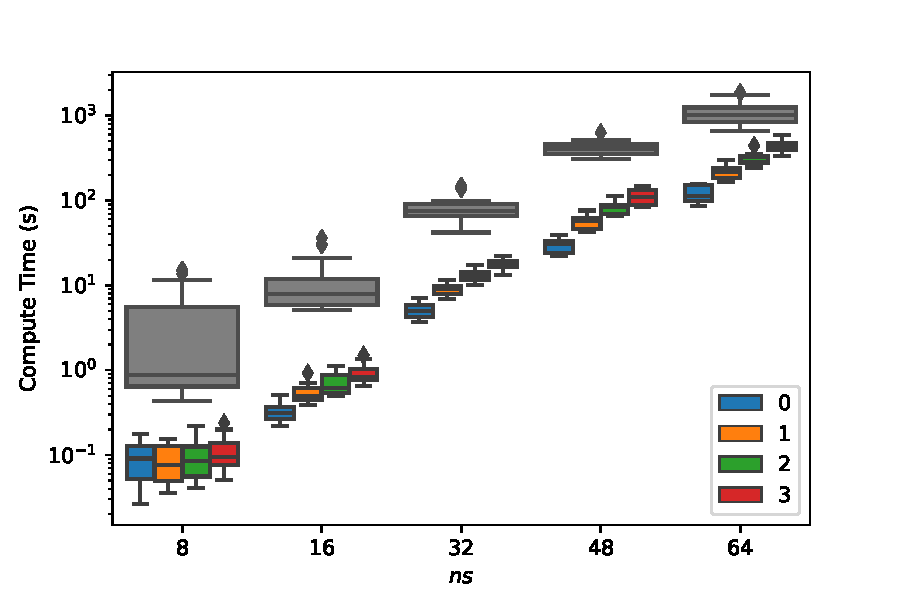
\includegraphics[width=5in]{compute_time_violin}
  \caption{mms asym err time. 32 cores.}
  \label{fig:compute_time_violin}
\end{figure}


\begin{figure}[H]
  \centering
  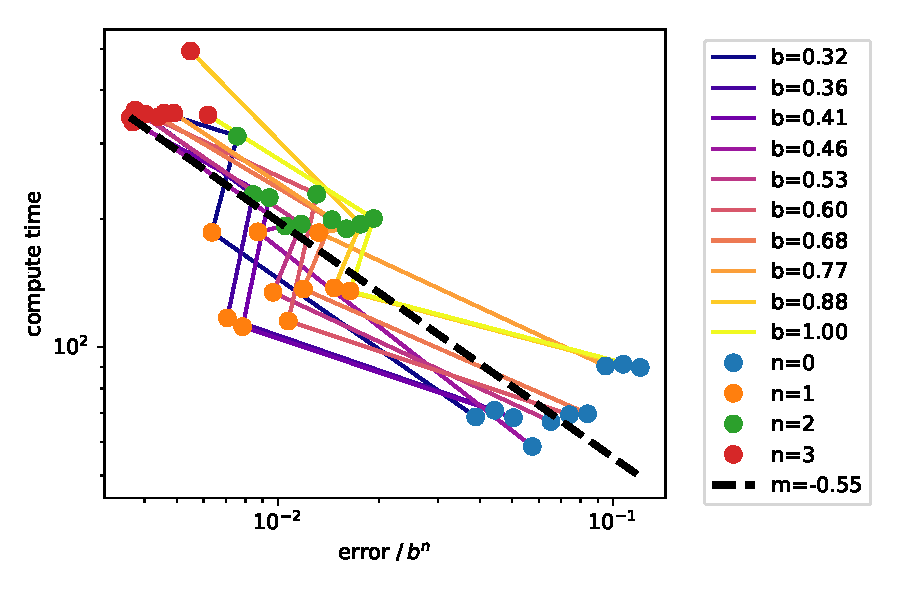
\includegraphics[width=5in]{mms_asym_err_time_collapsed}
  \caption{To give an idea of the trade--off between accuracy and speed; $n_s=64$, $n_a=8$. $\varepsilon t^2 \propto b^n$. 32 cores.}
  \label{fig:mms_asym_err_time_collapsed}
\end{figure}

\subsection{Memory Usage}
\begin{figure}[H]
  \centering
  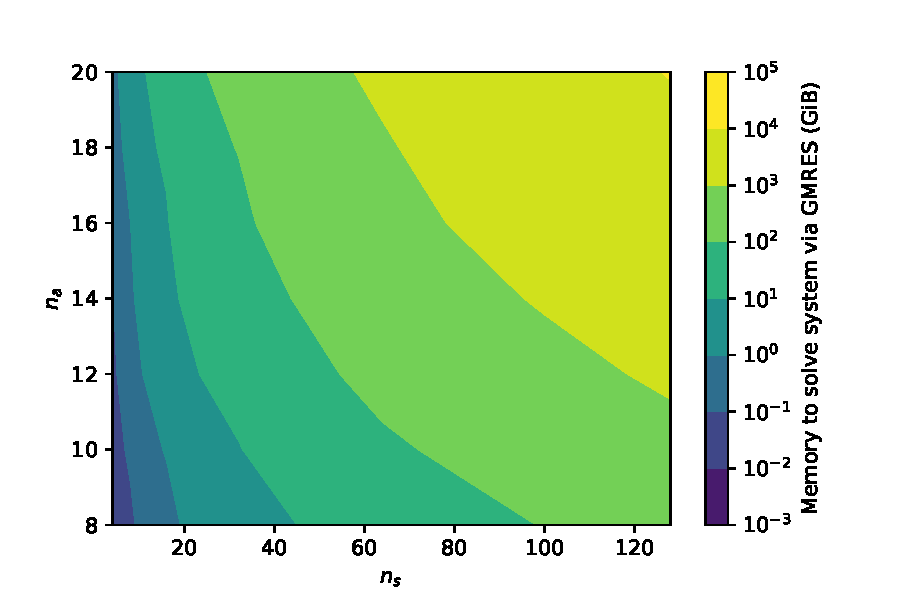
\includegraphics[width=5in]{memory_solve}
  \caption{Memory to solve the linear system of equations with GMRES restarted every 100 iterations. This seems to require roughly five times the memory required to store the matrix. See Table \ref{tab:mem_solve} for values.}
  \label{fig:memory_solve}
\end{figure}

%\section{Grid Size and Discretization Error}
\section{Optical Conditions for Asymptotics}

\subsection{Raw data}

\newcommand\rdfigwidth{4.5in}

\begin{figure}[H]
  \centering
  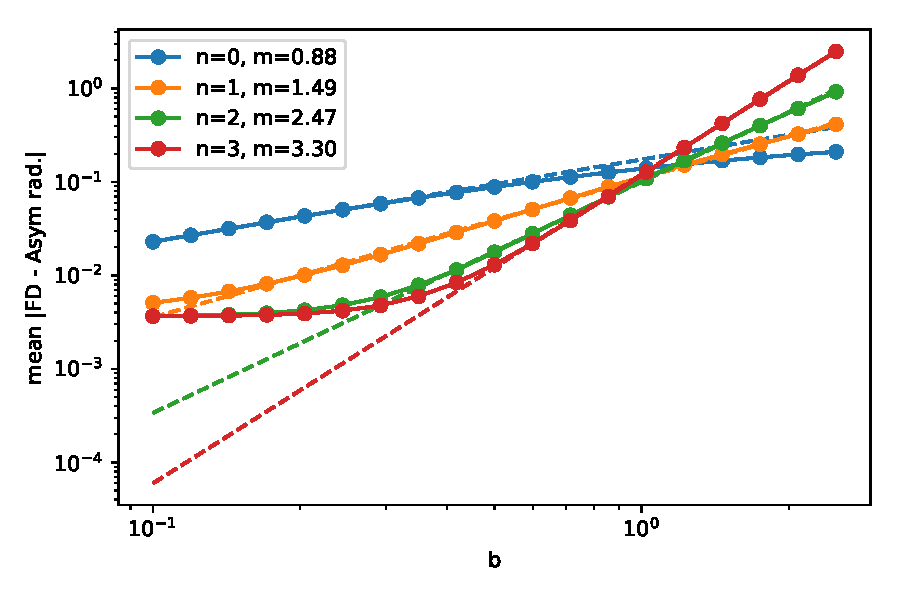
\includegraphics[width=\rdfigwidth]{verify_real_kelp_asym_b_scat_ss_sm_th_a05_br01_72x10_rad_err}
  \caption{Asym real kelp. Blur radius=0.1}
  \label{fig:asym_real_kelp_br01}
\end{figure}

\begin{figure}[H]
  \centering
  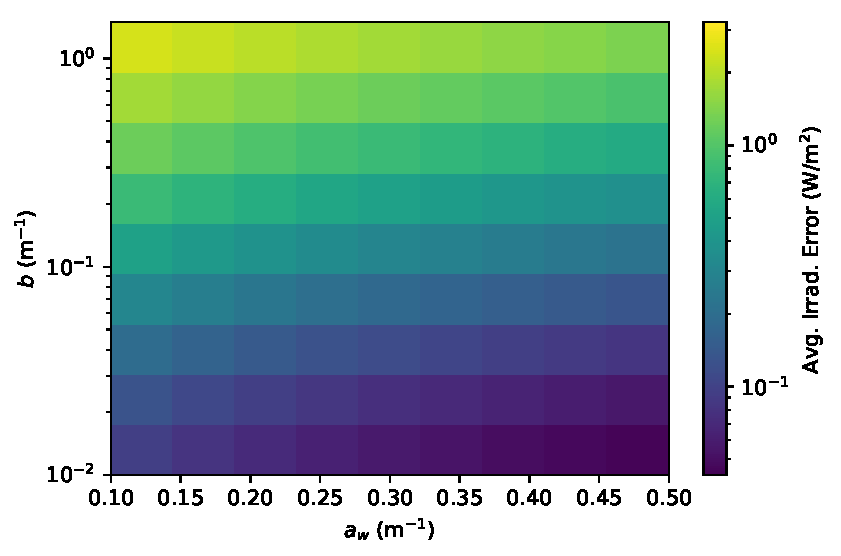
\includegraphics[width=\rdfigwidth]{asym_err_vs_ab}
  \caption{asym err vs ab}
  \label{fig:asym_err_vs_ab}
\end{figure}

\begin{figure}[H]
  \centering
  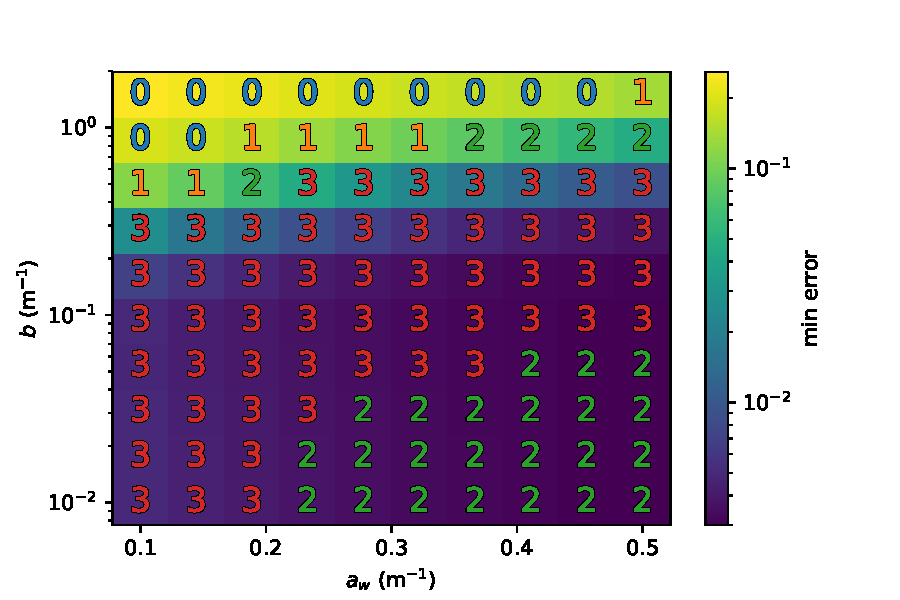
\includegraphics[width=\rdfigwidth]{best_n_data_vs_ab}
  \caption{best n data vs ab}
  \label{fig:best_n_data_vs_ab}
\end{figure}

\begin{figure}[H]
  \centering
  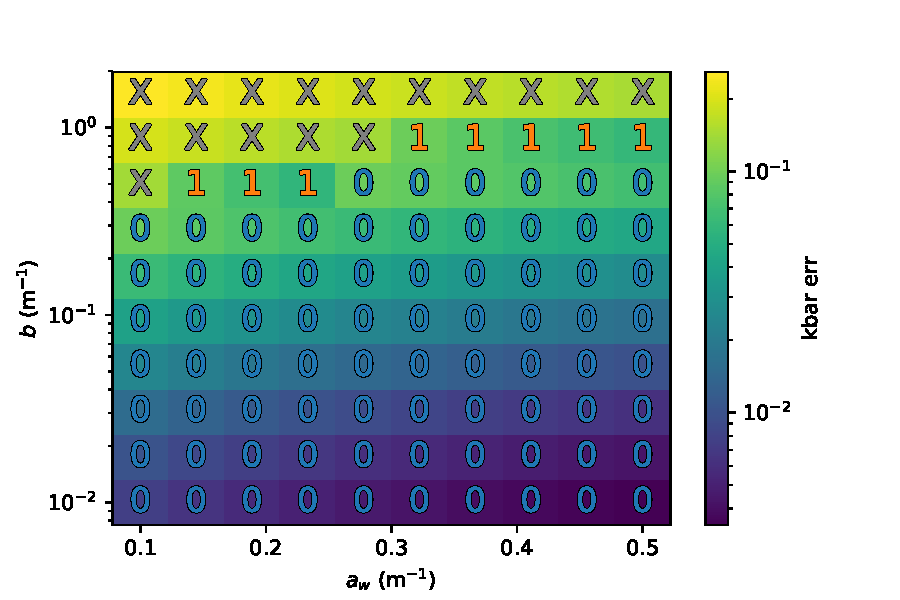
\includegraphics[width=\rdfigwidth]{min_n_data_vs_ab_eps01}
  \caption{min n data vs ab eps01}
  \label{fig:min_n_data_vs_ab_eps01}
\end{figure}

\begin{figure}[H]
  \centering
  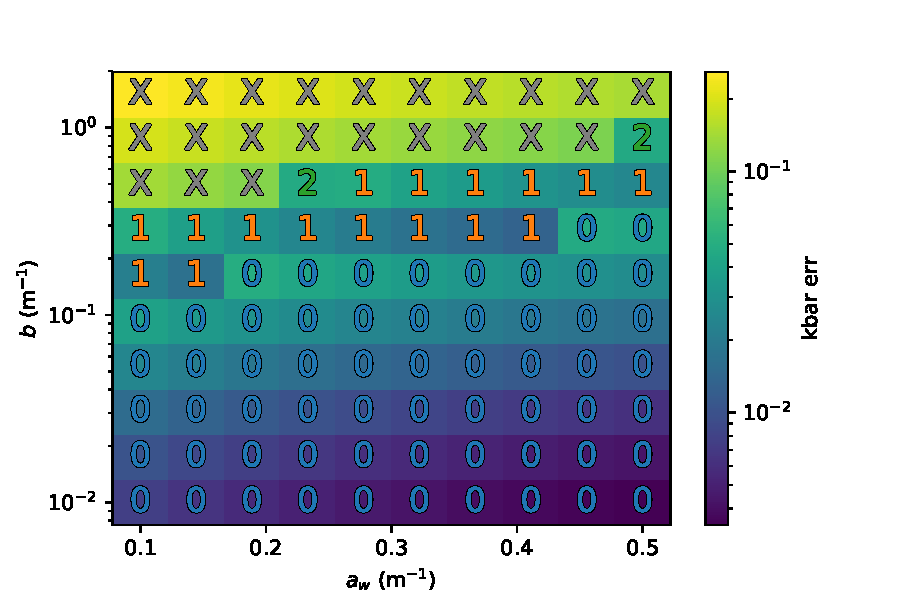
\includegraphics[width=\rdfigwidth]{min_n_data_vs_ab_eps005}
  \caption{min n data vs ab eps005}
  \label{fig:min_n_data_vs_ab_eps005}
\end{figure}

\begin{figure}[H]
  \centering
  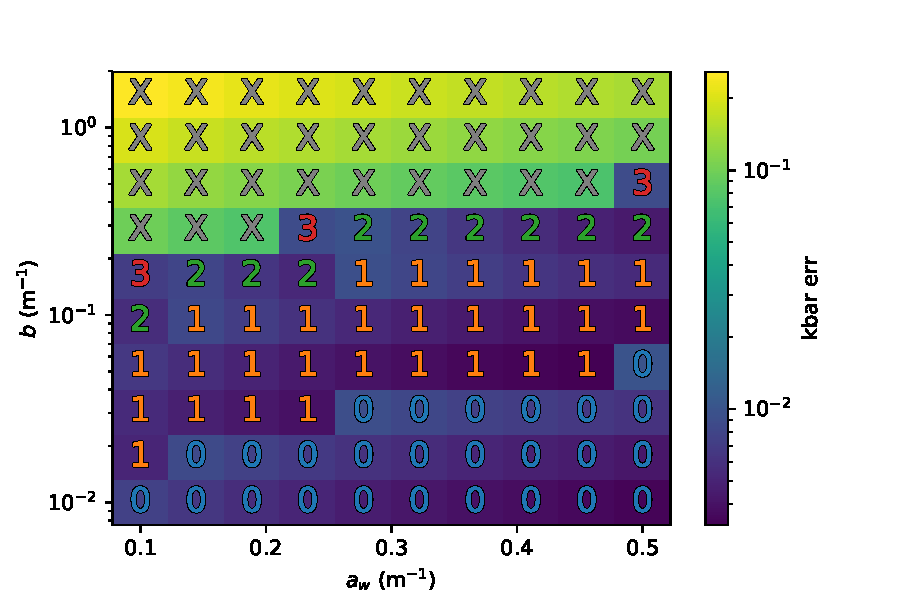
\includegraphics[width=\rdfigwidth]{min_n_data_vs_ab_eps001}
  \caption{min n data vs ab eps001}
  \label{fig:min_n_data_vs_ab_eps001}
\end{figure}

\subsection{Error Model}

\begin{figure}[H]
  \centering
  %\vspace{-1em}
  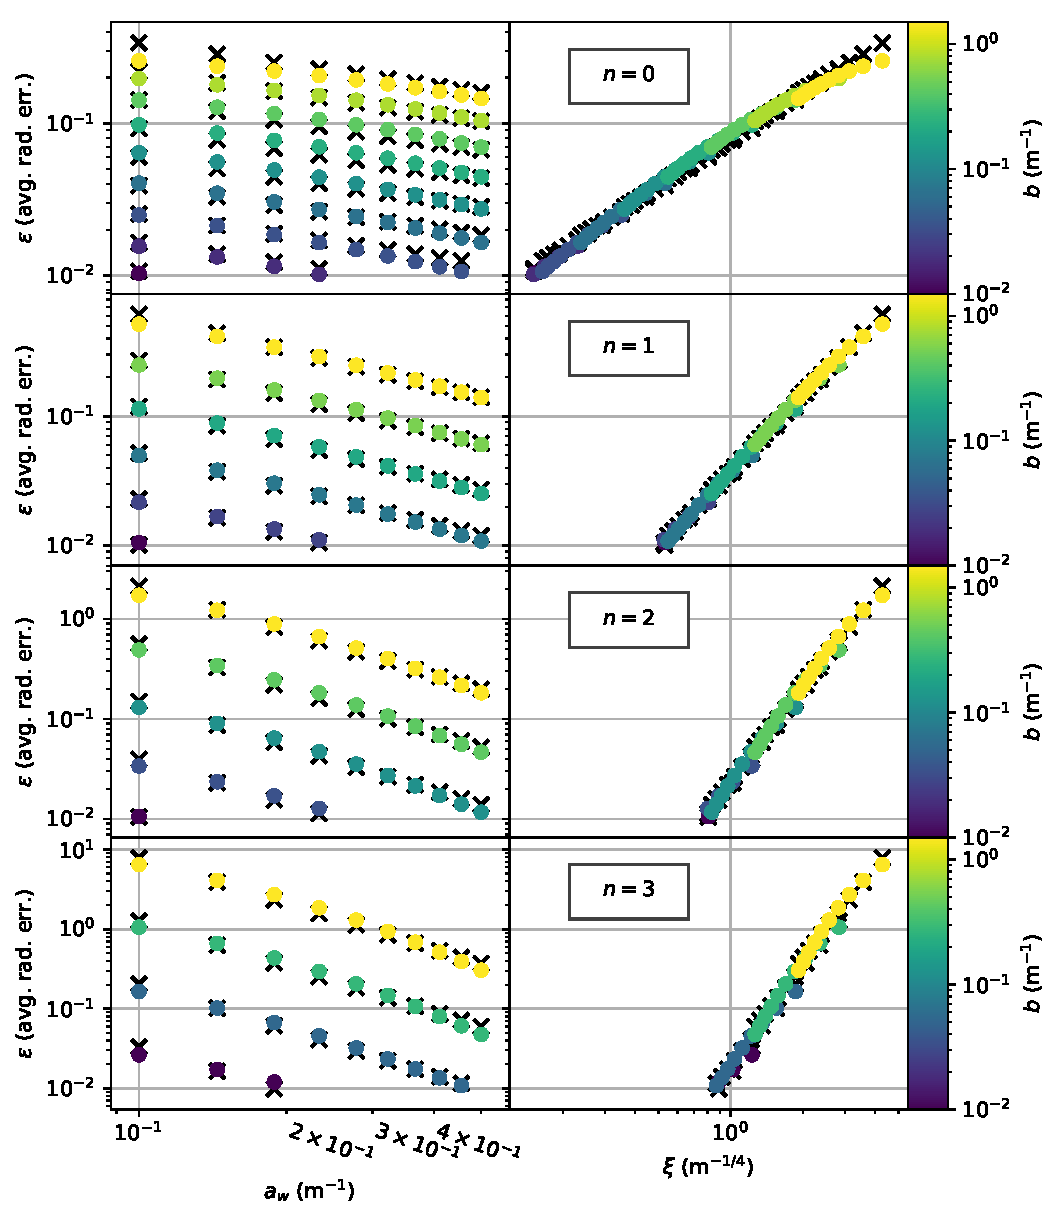
\includegraphics[width=5in]{asym_err_data_xi_model}
  %\vspace{-1em}
  \caption{asym err data xi model}
  \label{fig:asym_err_data_xi_model}
\end{figure}

\begin{figure}[H]
  \centering
  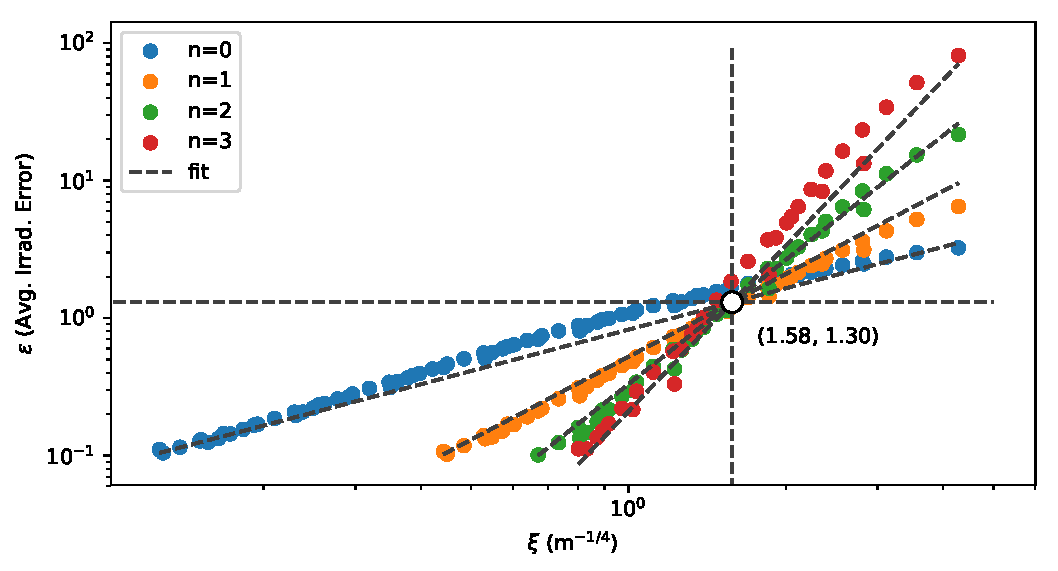
\includegraphics[width=5in]{asym_err_vs_xi_all_n_fit_all}
  \caption{asym err vs xi all n fit all}
  \label{fig:asym_err_vs_xi_all_n_fit_all}
\end{figure}

\begin{figure}[H]
  \centering
  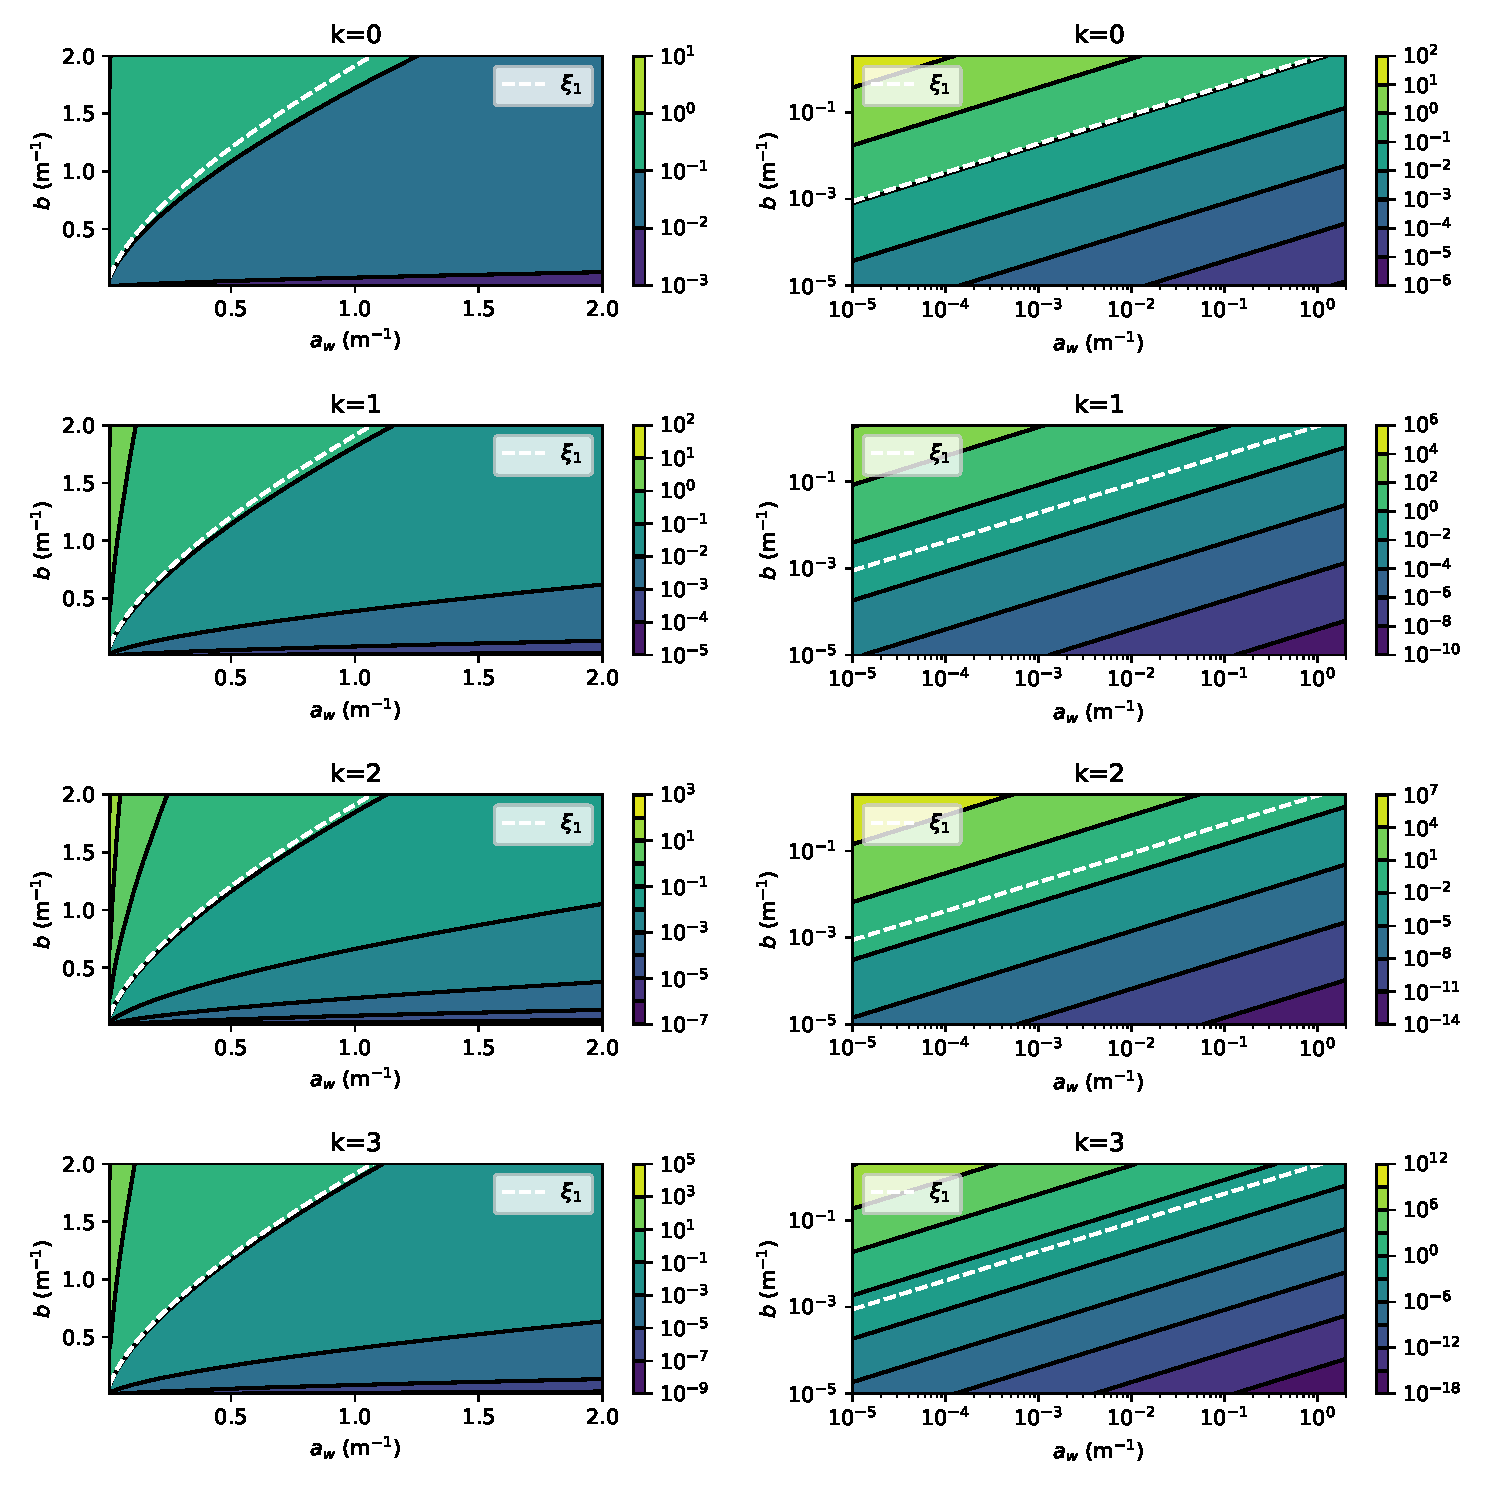
\includegraphics[width=5in]{asym_err_model_vs_ab_all_k}
  \caption{asym err model vs ab all k}
  \label{fig:asym_err_model_vs_ab_all_k}
\end{figure}

\begin{figure}[H]
  \centering
  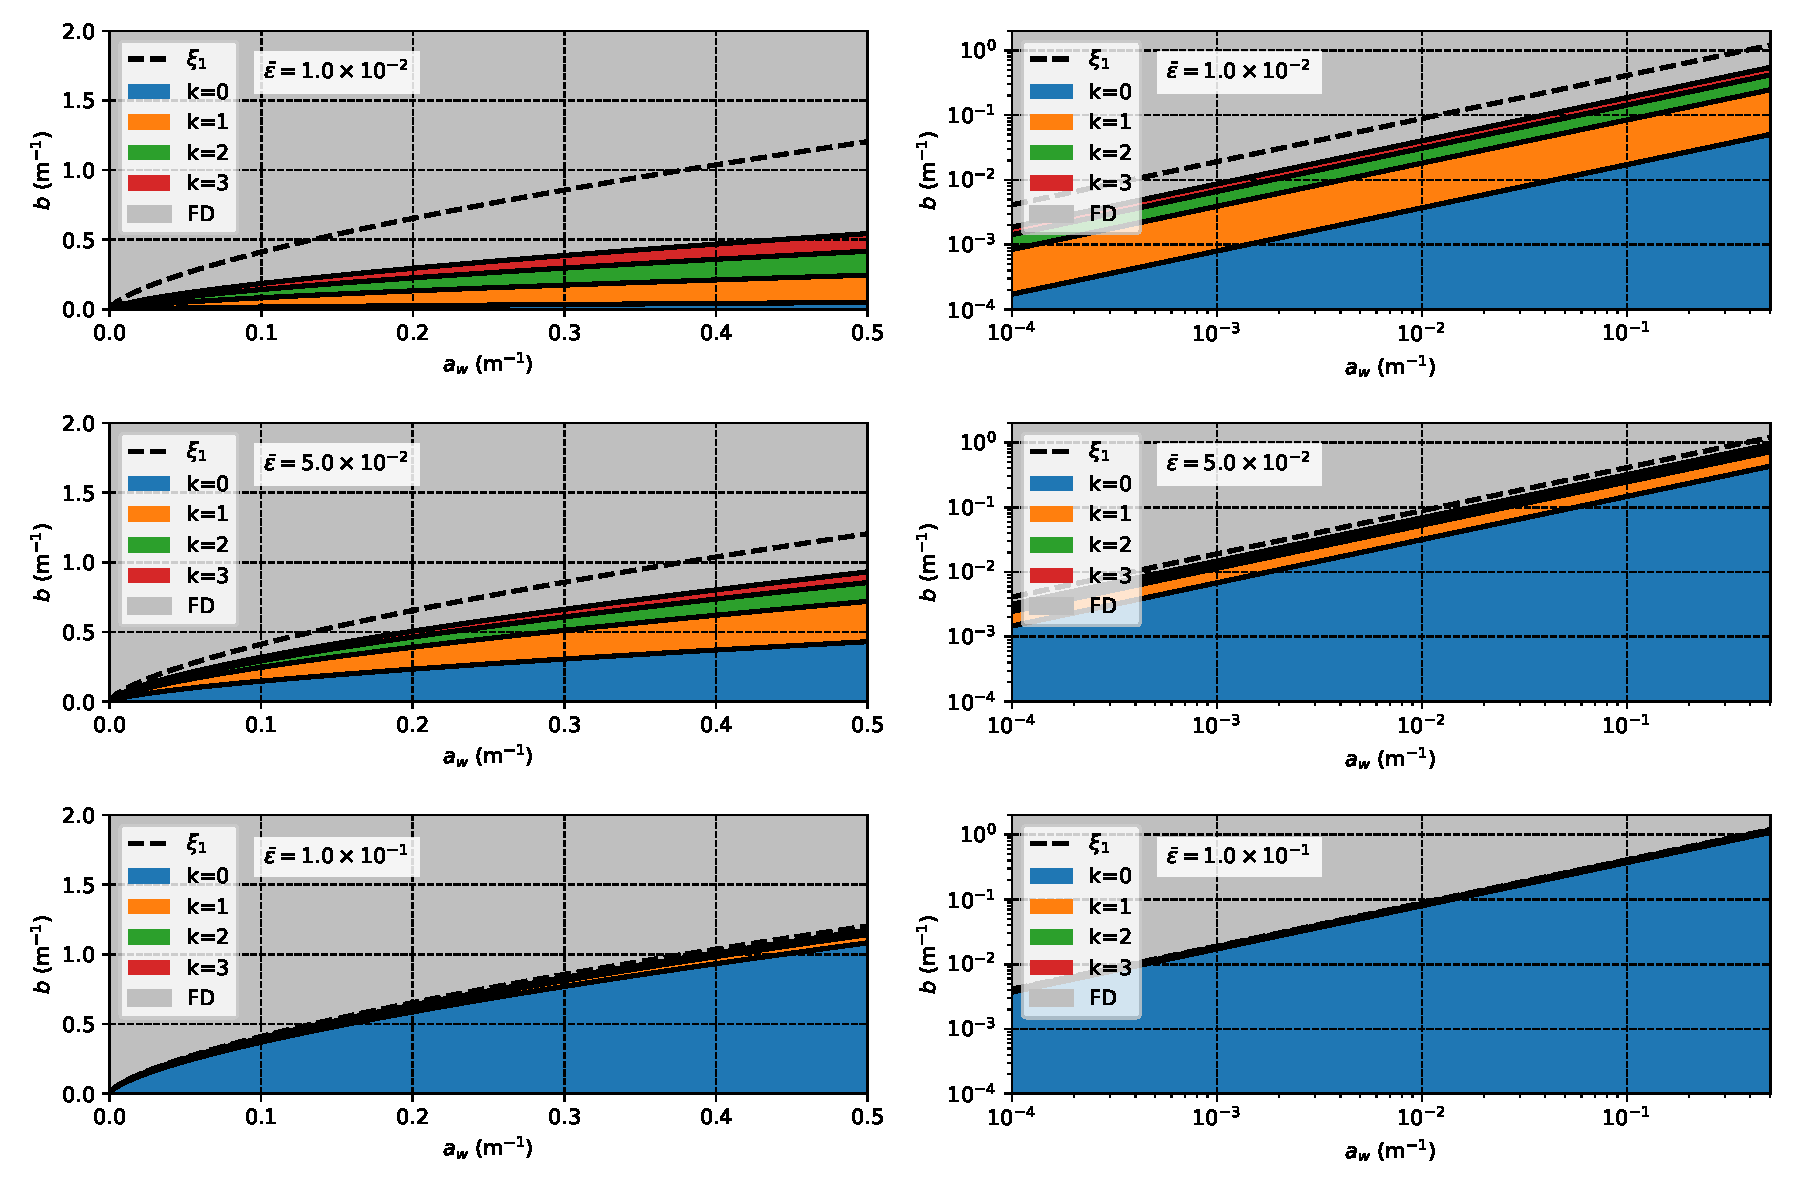
\includegraphics[width=5in]{nbar_model_vs_ab_3eps}
  \caption{nbar model vs ab 3eps}
  \label{fig:nbar_model_vs_ab_3eps}
\end{figure}


\section{Comparison to Other Light Models}

\subsection{Full 10m}
\begin{figure}[H]
  \centering
  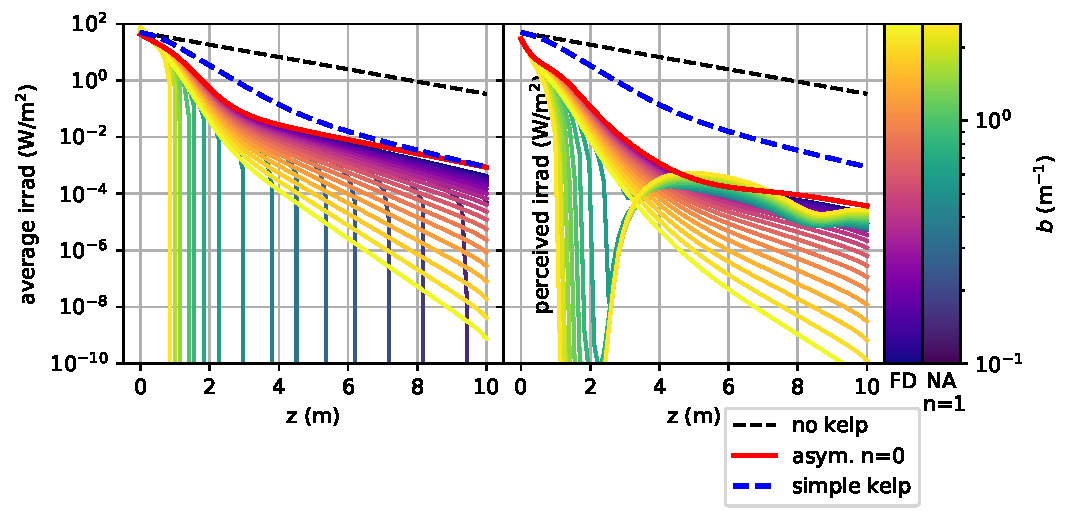
\includegraphics[width=6in]{compare_models_n1}
  \caption{Compare models n=1}
  \label{fig:compare_models_n1}
\end{figure}
\begin{figure}[H]
  \centering
  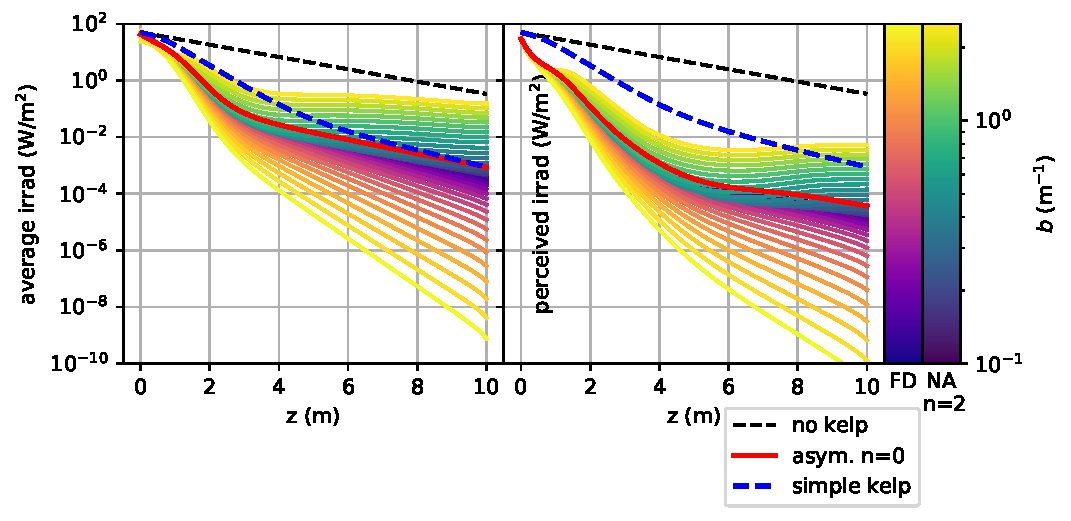
\includegraphics[width=6in]{compare_models_n2}
  \caption{Compare models n=2}
  \label{fig:compare_models_n2}
\end{figure}
\begin{figure}[H]
  \centering
  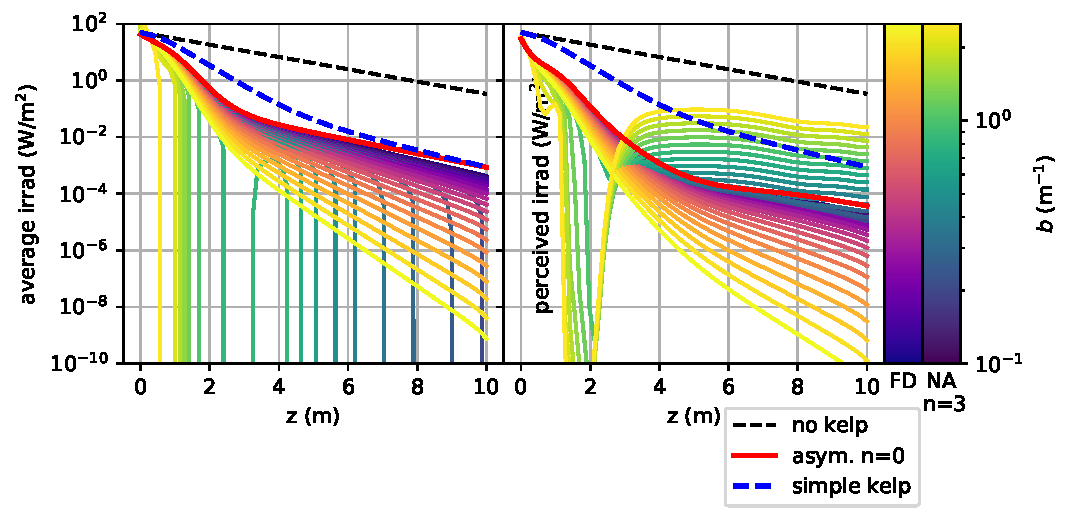
\includegraphics[width=6in]{compare_models_n3}
  \caption{Compare models n=3}
  \label{fig:compare_models_n3}
\end{figure}
